%!TEX root = ../username.tex
\chapter{Results and Future Work} \label{results_future}

\section{Results} \label{results}

% TODO add something here

\subsection{The LSTM Neural Network}

With the neural network setup described in Section \ref{software:ga:fitness}, the network is able to correctly predict whether a set of notes is Bach or not $99\%$ of the time.
This is the same whether it is trained on the Bach cello suites or the chorales provided by music21.
As described in Section \ref{software:ga:fitness}, fitness values are the output of a squashing function with the range $(0,1)$.
The input to the squashing function is the difference between how much the LSTM neural network thinks the melody is good and how much the network thinks it is bad.
Table \ref{table:fitnesscomp} contains the fitness values for music by Bach, Domenico Scarlatti, and Franz Joseph Haydn.
Two different versions of the fitness function were used; one trained on music21's Bach chorales, and the other on Bach cello suites.
As expected, the fast paced violin sonata by Haydn and the piano exercise by Scarlatti performed much better when using the fitness function trained with the cello suites, while the Little Fugue, which contains some longer rhythms performed better when the fitness function trained with the chorales.
This is expected because the cello suites are fast paced and the chorales have a slow pace.

\begin{figure}[]
	\centering
	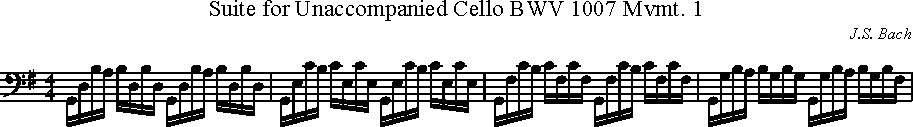
\includegraphics[width=\linewidth]{figures/cello_suite.pdf}
	\caption{Opening of the first movement of the first Cello Suite by J.S. Bach.}
	\label{fig:music:cello_suite}
\end{figure}

\begin{figure}[]
	\centering
	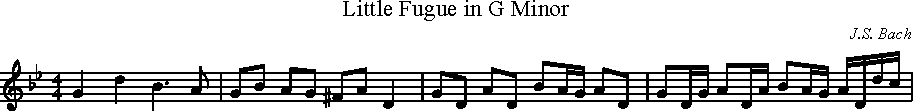
\includegraphics[width=\linewidth]{figures/little_fugue.pdf}
	\caption{Little Fugue in G Minor by J.S. Bach.}
	\label{fig:music:little_fugue}
\end{figure}

\begin{figure}[]
	\centering
	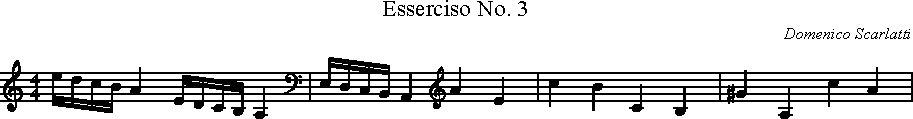
\includegraphics[width=\linewidth]{figures/scarlatti.pdf}
	\caption{Piano Exercise by Domenico Scarlatti.}
	\label{fig:music:scarlatti}
\end{figure}

\begin{figure}[]
	\centering
	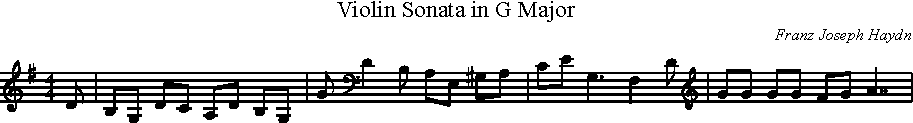
\includegraphics[width=\linewidth]{figures/haydn.pdf}
	\caption{Violin Sonata in G Major by Franz Joseph Haydn.}
	\label{fig:music:haydn}
\end{figure}

See Figures \ref{fig:music:cello_suite}, \ref{fig:music:little_fugue}, \ref{fig:music:scarlatti}, and \ref{fig:music:haydn} for the samples from the pieces that were tested for their fitnesses.

\begin{table}[]
	\centering
	\begin{tabular}{c | c c}
		Piece & Fitness (Chorales) & Fitness (Cello Suites) \\
		\hline
%		J.S. Bach Cello Suite 1, Mvmt. 1 & $0.15419$ & $0.90229$ \\
		J.S. Bach Little Fugue in G Minor & $0.87171$ & $0.86847$ \\
		Domenico Scarlatti & $0.23755$ & $0.92652$ \\
		Haydn Violin Sonata & $0.77070$ & $0.91706$
	\end{tabular}
	\caption{Fitness values of music by various authors using models trained with music21's Bach chorales and Bach's cello suites}
	\label{table:fitnesscomp}
\end{table}

\subsection{Markov Chains vs Random Notes}
Although the initial population's fitness is generally greater when using Markov chains create the melodies, the use of the genetic algorithm quickly negates that difference within a few generations.
Figures \ref{fig:fitness_markov} and \ref{fig:fitness:random} show the top fitness values from the population for the first 50 generation of a run of the program.
The first figure's initial population was generated by Markov chains, and the second figure's initial population was randomly generated.
The initial fitness and fitness of the first several generations starts higher in the first figure, but after about the fifth generation, the fitness in the second figure matches, and eventually surpasses, that of the first.
So the fitness of the randomly seeded population can quickly surpass the fitness of the Markov chain seeded population.
Thus, since the time to generate the initial population using Markov chains is considerable, compared to using list comprehensions to create random notes, the Markov chain melodies should probably be relegated to generating one-off melodies.

\begin{figure}[h]
	\centering
	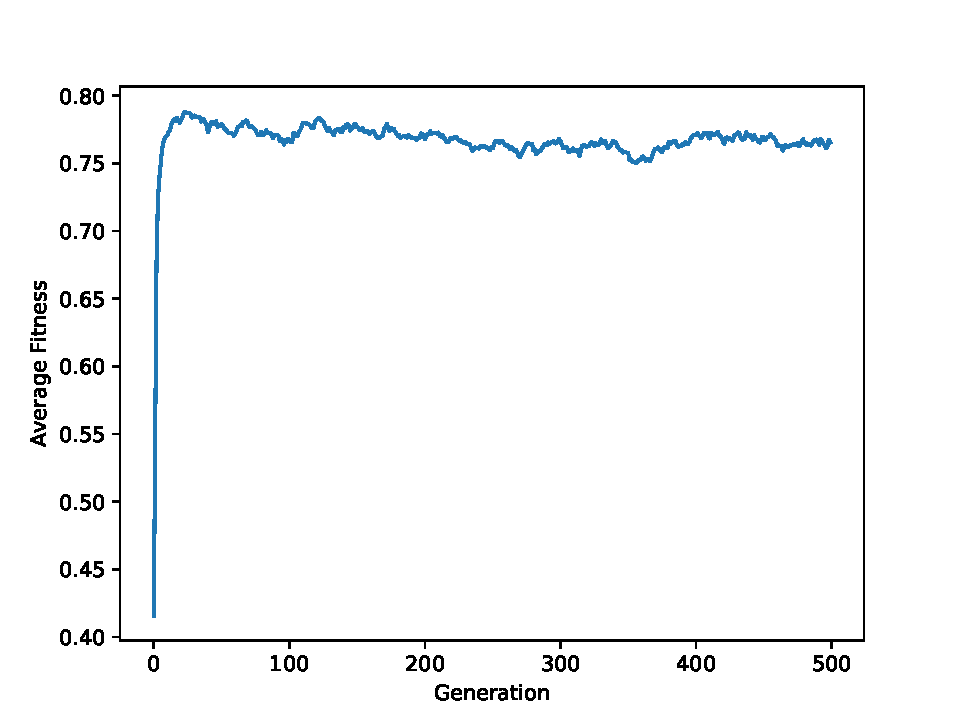
\includegraphics[width=\linewidth]{fitnesses_markov_start.pdf}
	\caption{Fitness over 50 generations with an initial population generated using Markov chains.}
	\label{fig:fitness_markov}
\end{figure}

\begin{figure}[h]
	\centering
	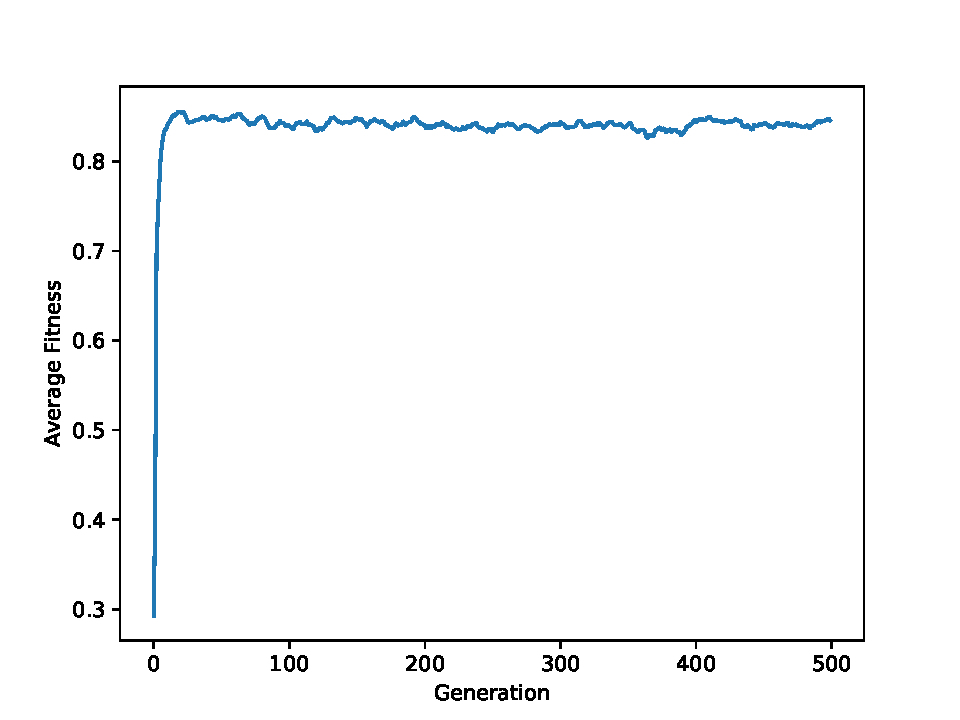
\includegraphics[width=\linewidth]{figures/fitnesses_random_start.pdf}
	\caption{Fitness over 50 generations with a random initial population.}
	\label{fig:fitness:random}
\end{figure}

\subsection{The Music and Its Uses}

\begin{figure}[h]
	\centering
	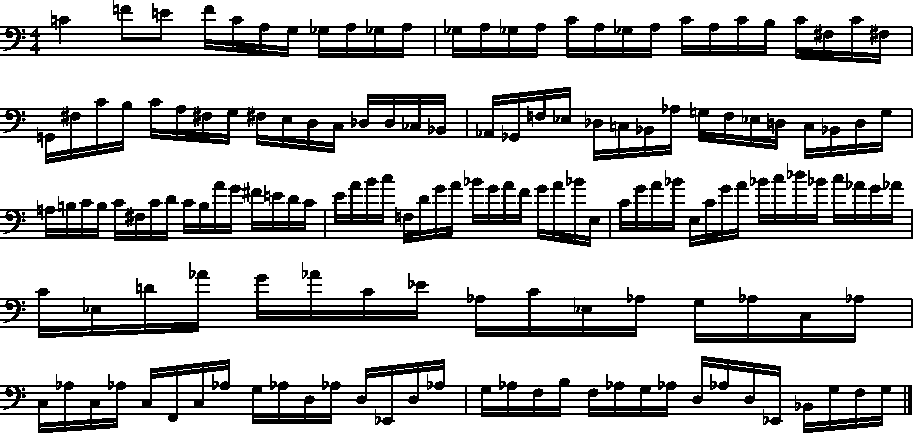
\includegraphics[width=\linewidth]{figures/markov_melody_1.pdf}
	\caption{A melody generated by Markov chains.}
	\label{fig:music:markov1}
\end{figure}

\begin{figure}[h]
	\centering
	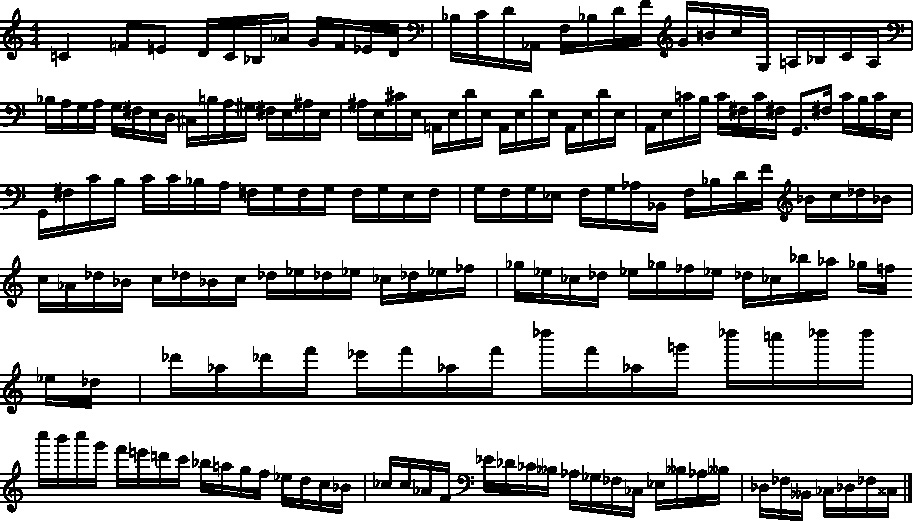
\includegraphics[width=\linewidth]{figures/markov_melody_2.pdf}
	\caption{A melody generated by Markov chains.}
	\label{fig:music:markov2}
\end{figure}

Figures \ref{fig:music:markov1} and \ref{fig:music:markov2} show two melodies generated using Markov chains.
They were generated using a third order Markov chain for the intervals between notes and a second order Markov chain for the rhythms.
Of particular interest, the second measure of the second line of Figure \ref{fig:music:markov2} contains a figure repeated three times.
Additionally, the first measure of the last line of that particular melody contains a perfect run down the B$\flat$ Major scale (from B$\flat$5 to B$\flat$4) in its last two beats.
With the exception of the $E6$ in the second beat of this measure not being an E$\flat$, it is almost a perfect run down the scale starting on G6 and ending on B$\flat$4.

\begin{figure}[h]
	\centering
	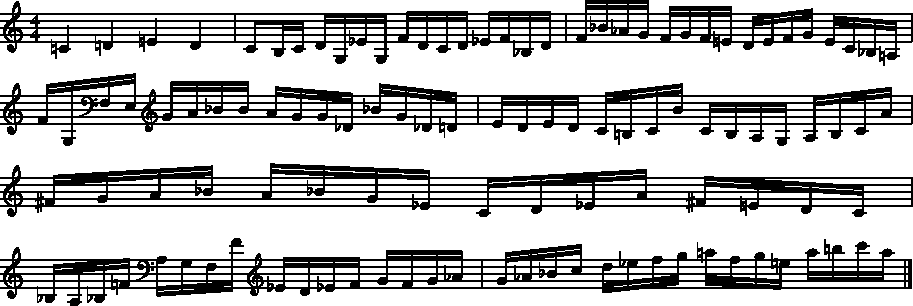
\includegraphics[width=\linewidth]{figures/markov_melody_3.pdf}
	\caption{A melody generated by random order Markov chains.}
	\label{fig:music:markov3}
\end{figure}

\begin{figure}[h]
	\centering
	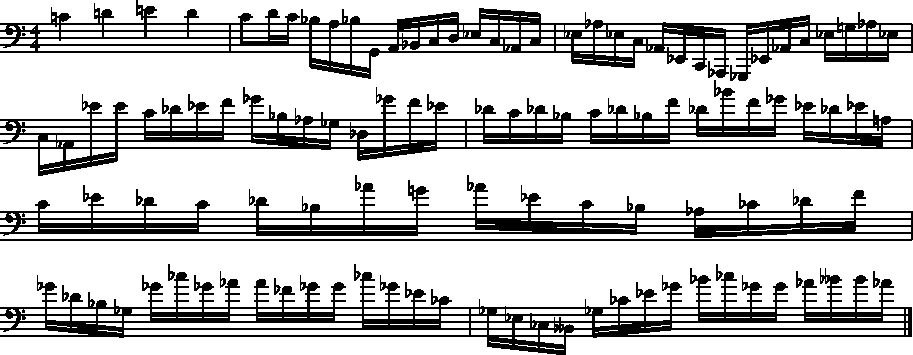
\includegraphics[width=\linewidth]{figures/markov_melody_4.pdf}
	\caption{A melody generated by random order Markov chains.}
	\label{fig:music:markov4}
\end{figure}

Figures \ref{fig:music:markov3} and \ref{fig:music:markov4} contain melodies that were generated using random order Markov chains, meaning the order to determine intervals between notes and the order to determine rhythm were selected at random from the range $1$ through $5$.
Something of interest that occurs in Figure \ref{fig:music:markov3} is that after the initial four notes, which were provided by the author, the rest of the melody is almost in C Minor.
In general we expect most of the pieces produced to tend toward C Major or A Minor, as those are the keys the Markov model was trained on.
Even though the melody shifted from the expected key, it manages to maintain coherence because the music the Markov chain was trained with stay in one key, and so too does the produced melody.

\begin{figure}[h]
	\centering
	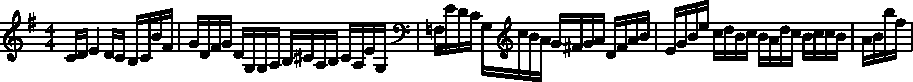
\includegraphics[width=\linewidth]{figures/genetic_melody_1.pdf}
	\caption{A melody generated with the genetic algorithm.}
	\label{fig:music:genetic1}
\end{figure}

\begin{figure}[h]
	\centering
	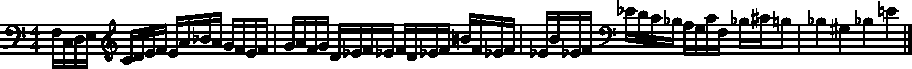
\includegraphics[width=\linewidth]{figures/genetic_melody_2.pdf}
	\caption{A melody generated with the genetic algorithm.}
	\label{fig:music:genetic2}
\end{figure}

The melodies is Figures \ref{fig:music:genetic1} and \ref{fig:music:genetic2} were generated using the genetic algorithm with the surrogate fitness function trained using the chorales from music21's built in corpus of Bach music and an initial population of randomly generated melodies.
Of particular interest in Figure \ref{fig:music:genetic1} is the set of arpeggiations in the third and fourth measures.
Without explicitly telling the algorithm anything about arpeggios or repeating ideas in slightly differing ways, it picked up that this makes for good (Bach-like) music.

\begin{figure}[h]
	\centering
	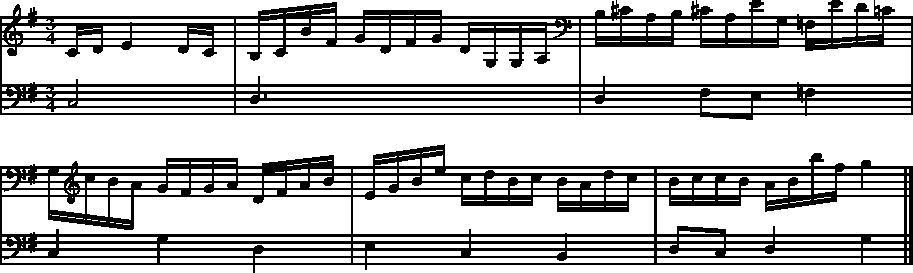
\includegraphics[width=\linewidth]{figures/genetic_melody_1_harmonized.pdf}
	\caption{The melody in Figure \ref{fig:music:genetic1} with a bass line written by the author.}
	\label{fig:music:geneticHarmonized}
\end{figure}

An application of this project is to provide inspiration for the composer.
See Figure \ref{fig:music:geneticHarmonized} for an example where the author used the melody from Figure \ref{fig:music:genetic1} and added a bass line and more satisfying ending.
The generated melodies could also be chained together to create longer compositions, or they could have their rhythms increased by some multiple to have more than a snippet of music.

The ambitious musician might use these melodies to practice their sight reading; it is extremely unlikely that a melody produced by either the Markov chains or genetic algorithm has even been written before, let alone seen by a particular musician.
Therefore, these melodies could provide a great opportunity to practice reading music seen for the first time.

\section{Future Work} \label{future}

The work in this project could be expanded by writing code to generate counterpoint or harmonizations of melodies that are created through this project.
One possible method to do this might involve simply using music21's ability to create a \textit{Roman numeral analysis} (RNA) of a piece to determine which chords to use.
Then, the software could fill in the bass, tenor, and alto parts with notes that fit the RNA.
This would likely create very simple, possibly boring, harmonies that may not follow all the voice leading rules of Western music.
But it would create \textit{a} complete harmonization.

Many authors have written about the topic of automatic harmonization.
Interestingly, much of the research on this topic focuses on using genetic algorithms to accomplish the task.
William Schottstaedt \cite{schottstdaet_automatic_1989} defines a genetic algorithm to generate multi-voice music that follows the rules of the Common Practice era.
Somnuk Phon-Amnuaisuk and Geraint A. Wiggins \cite{phon-amnuaisuk_four-part_1999} use genetic algorithms to harmonize preexisting soprano parts.
Andres Acevedo \cite{acevedo_fugue_2004} uses genetic algorithms to write counterpoint in a fugue setting.
A fugue is a musical form in which an initial theme is introduced in one part, that is imitated in other parts and repeated throughout the piece.
There are many other examples of using genetic algorithms to solve harmonization and counterpoint; these are just a small sample of the approaches explored.

Approaches other than using genetic algorithms also exist for creating pleasing counterpoint.
For example, David Cope discusses a rule-based approach to writing counterpoint \cite{cope_computers_1991}.
In this method, a set of rules about how to compose is provided to the program, rather than the program learning from the music on which it is based.
In another approach, Kamil Adiloglu and Ferda Alpaslan \cite{adiloglu_machine_2007} use a feed forward neural network to accept a single voice melody and produce a second voice to complement the first one.

Along with adding counterpoint or harmony generation, one might take different approaches to produce melodies.
For example, Chun-Chi Chen and Risto Miikkulainen \cite{chen_creating_2001} combine neural networks and genetic algorithms by using an evolutionary algorithm to find neural networks that produce good melodies.
